


\begin{figure}[H]
\caption{Lote de tareas ejecutando con Round Robin con quantum 2}
\label{fig:ej5q2}
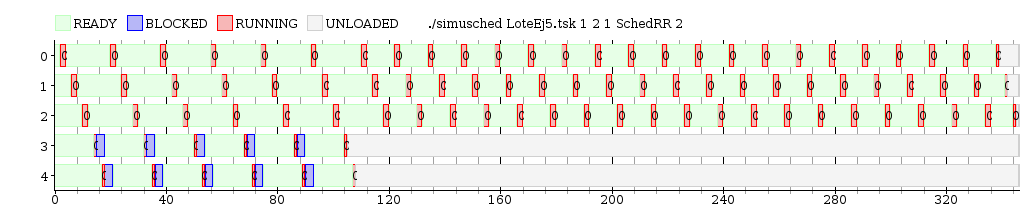
\includegraphics[width=1\textwidth]{imgs/ej5-q2.png}
\end{figure}


\begin{figure}[H]
\caption{Lote de tareas ejecutando con Round Robin con quantum 10}
\label{fig:ej5q10}
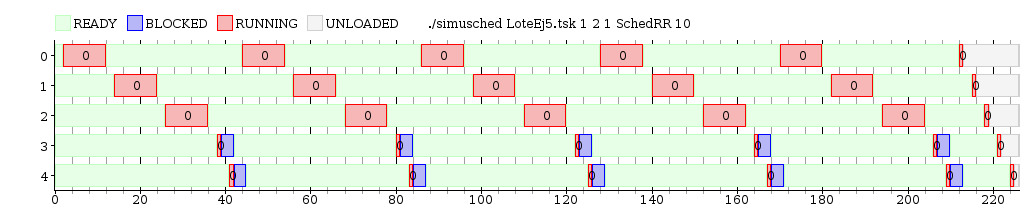
\includegraphics[width=1\textwidth]{imgs/ej5-q10.png}
\end{figure}


\begin{figure}[H]
\caption{Lote de tareas ejecutando con Round Robin con quantum 50}
\label{fig:ej5q50}
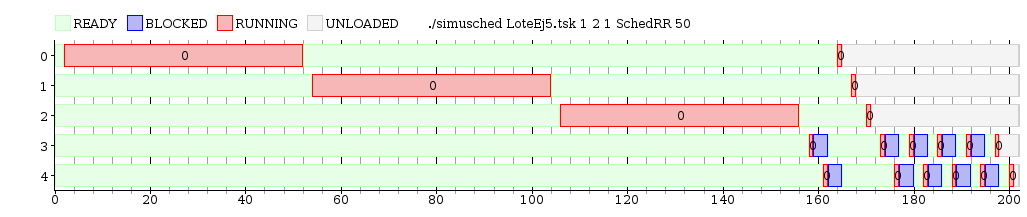
\includegraphics[width=1\textwidth]{imgs/ej5-q50.png}
\end{figure}

\begin{tabular}{| l | c | c | c |}
\hline  
\textbf{Quantum} & \textbf{2} & \textbf{10} & \textbf{50} \\ \hline
Latencia &  &  &  \\ \hline
Waiting Time &  &  &  \\ \hline
Tiempo Total &  &  &  \\ \hline
\end{tabular}


